\documentclass{article}

%Packages
\usepackage{graphicx}
\usepackage{grffile}
\usepackage{float}

%Margins
\usepackage[
	margin=2cm,
	includefoot
	]{geometry}

%Images
\usepackage{graphicx}

\graphicspath{{images/}}

%Headers and Footers
\usepackage{fancyhdr}
\pagestyle{fancy}
\fancyhead{}
\fancyfoot{}
\fancyfoot[R]{\thepage}
\renewcommand{\headrulewidth}{0pt}
\renewcommand{\footrulewidth}{0pt}


%Details
\title{
Software Requirements Specification and 
Technology Neutral Process Design
(University of Pretoria - software engineering COS301)
}
\date{2016-07-29}
\author{now.next();}

%Document start
\begin{document}

%Title Page
\begin{titlepage}
	\begin{center}
		
\includegraphics[width=10cm]{UP.jpg}  \\
		[1cm]
		\line(1,0){300} \\
		[0.4cm]
		\textsc{\huge
			Software Requirements Specification and 
			Technology Neutral Process Design
			(University of Pretoria - software engineering COS301)
		} \\
		[0.1cm]
		\line(1,0){300} \\
		[0.4cm]
		\textsc{\Large
			now.next();		} \\

	\end{center}
	\begin{flushright}
	\textsc{\Large
	Aiden Malan\\ 
	u12265731\\
	Vuyani Shabangu\\
	u11171139\\
	Sibusiso Masemola\\ 
	u12270467\\
	Sello Thosago\\
	u13062060\
	}
	\end{flushright}
\end{titlepage}

%Table of contents
\tableofcontents
\thispagestyle{empty}
\cleardoublepage

%Content
\setcounter{page}{1}
\section{Introduction}
%\lable{sec:intro} for some readon i cant get the lables to work maybe you guys will have some luck
The purpose of this document is to describe the requirements of the “Postgraduate Paper Interaction Portal” application, by illustrating the purpose and uses of the system, as well as the development of the system. The system constraints, interface and various interactions will also be discussed, and testable quality requirements will be provided where applicable.

\section{Vision}
	The project aims to equip people who see a need for a drone. Without having to own a very expensive drone or have the expertise to operate the drone which can be as expensive to acquire. With the Drone Mission Project in full effect customers can achieve maximum output out of every mission while the business continues to reap in the rewards of the service portal we provide.

\section{Background}
	The Drone Mission project is aimed at equipping a client that would need the services of the drone but does not own a drone or the expertise to control the drone. The client or user would register to the website service and request the details of his mission such as time, place and if it is a recurring mission every hour, day, week, etc. The system would process all details and a drone operator will send information back to system to fly the drone. Information is captured and sent to the client efficiently.

\section{Functional requirements and application design}
%\lable{sec:funcreq}
We will now speak on the different subsystems and show the use cases, service contracts, required functionality and process specifications. Our subsetions that we will focus on is the operator, mission and the user as these are the main subsections that make our project.

\subsection{Operator subsystem}
	\subsubsection{Use cases}

		\begin{flushleft}
			\textbf{Critical}
				\begin{itemize}
	  				\item Add drone
	  				\item Remove drone
				\end{itemize}
			\section{}
			Critical cases in our operator subsystem exist because the operator needs to assign drones to himself so that our system knows what operator has the type of drone we need.
			\textbf{Nice-To-Have}
				\begin{itemize}
	  				\item Edit drone
				\end{itemize}
			\section{}
			Editing a drone is considered nice to have as it would not cause any problems to the system if it was left out but it would make the system more flexible and user friendly.
		\end{flushleft}

	\subsubsection{Services Contracts}
		\section{}
		Our service contracts for the operator subsystem all requests consist of a drone state with 4 attributes namely model, fly time, capabilities and manufacturer. All responses happen to the drone. All pre conditions have the operator in power with post conditions being operations done on the database for the drone.
		\begin{figure}[H]
			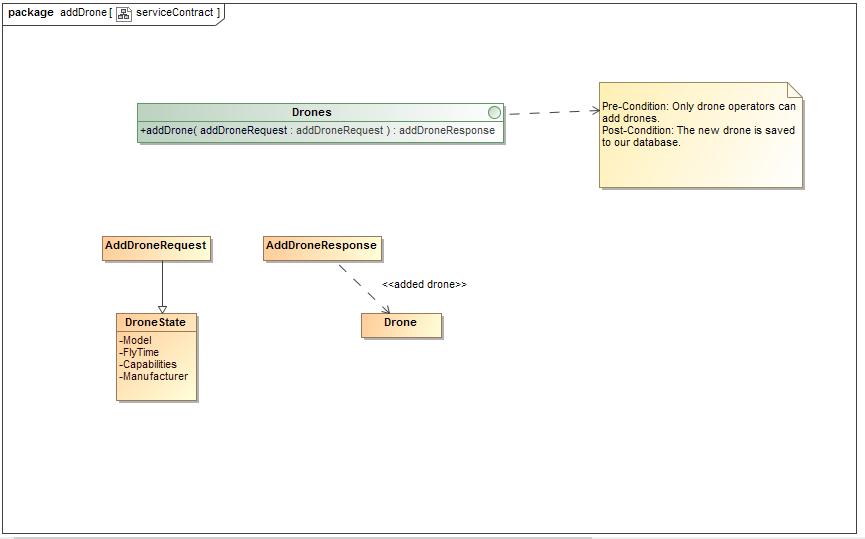
\includegraphics[width=\textwidth]{SC_add.png}  \\
			\caption{Services Contract : addDrone}
		\end{figure}
		\begin{figure}[H]
			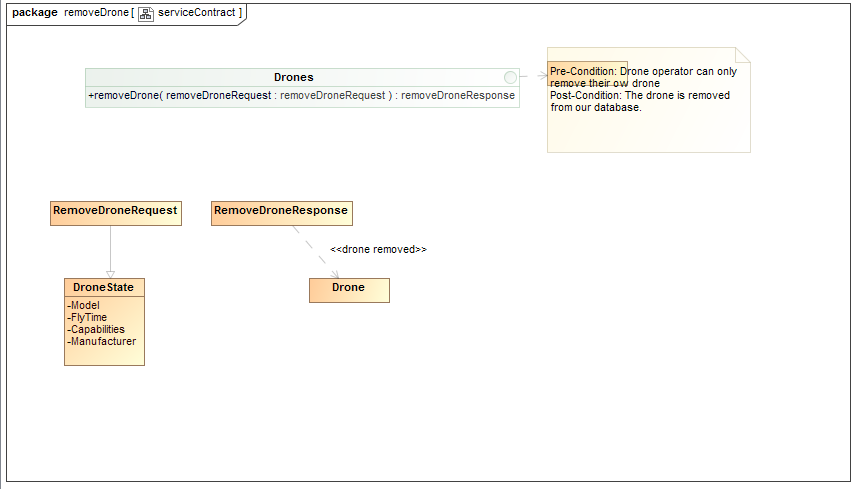
\includegraphics[width=\textwidth]{sc_delete.png}  \\
			\caption{Services Contract : removeDrone}
		\end{figure}
		\begin{figure}[H]
			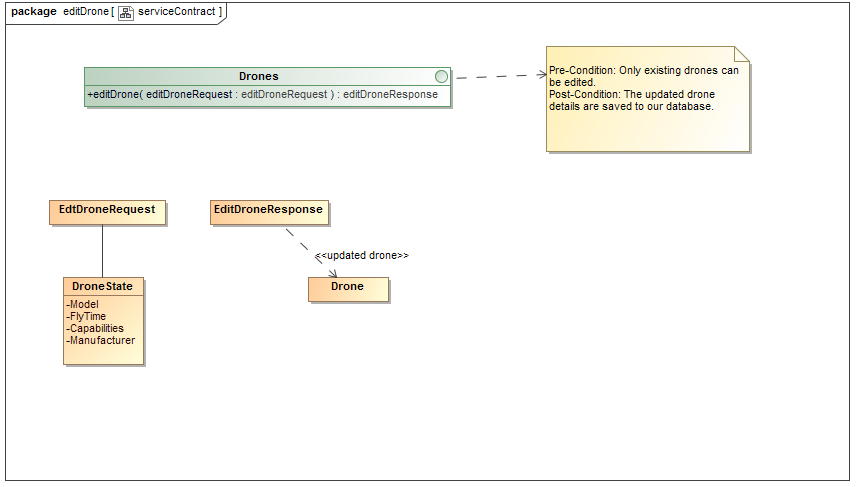
\includegraphics[width=\textwidth]{sc_edit.png}  \\
			\caption{Services Contract : editDrone}
		\end{figure}

	\subsubsection{Required functionality}
	The required functionality for the add drone, remove drone and edit drone functions are specified as follows:
		\begin{figure}[H]
			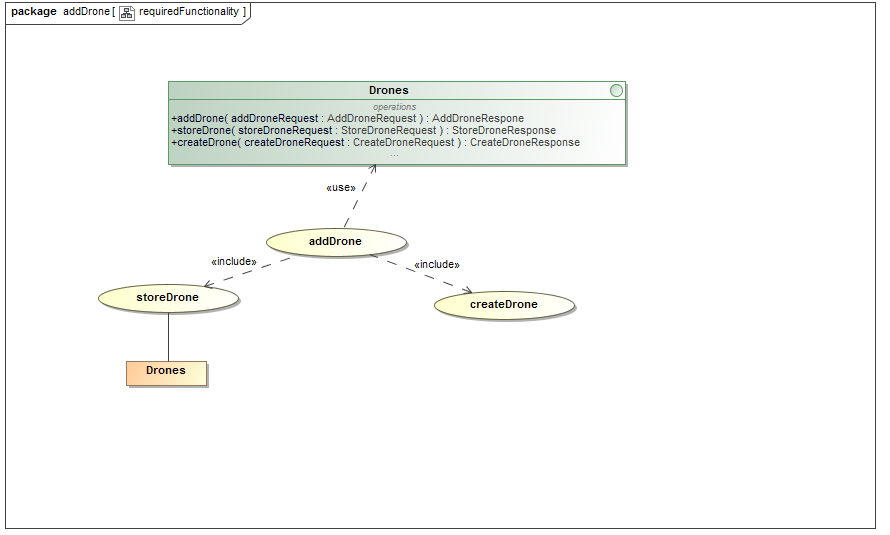
\includegraphics[width=\textwidth]{rf_add.png}  \\
			\caption{Functional Requirements : addDrone}
		\end{figure}
		\begin{figure}[H]
			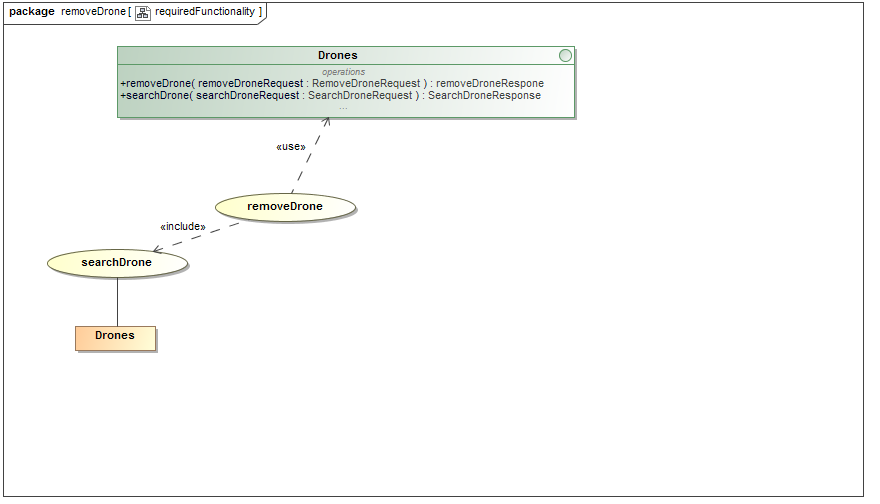
\includegraphics[width=\textwidth]{rf_remove.png}  \\
			\caption{Functional Requirements : removeDrone}
		\end{figure}
		\begin{figure}[H]
			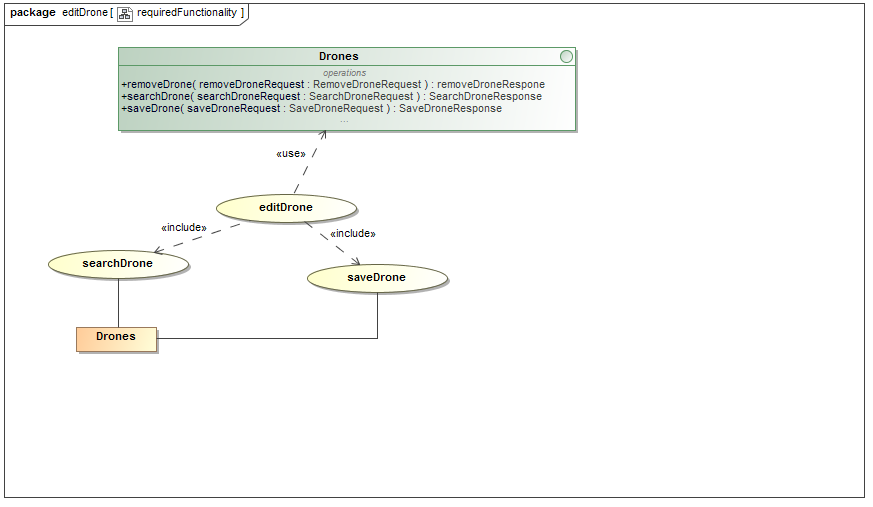
\includegraphics[width=\textwidth]{rf.png}  \\
			\caption{Functional Requirements : editDrone}
		\end{figure}
	

	\subsubsection{Process specifications}
	The process specifications describes the process that will be followed when the functions will executed. All processes require the drone to make changes to the database or throw an exception.
		\begin{figure}[H]
			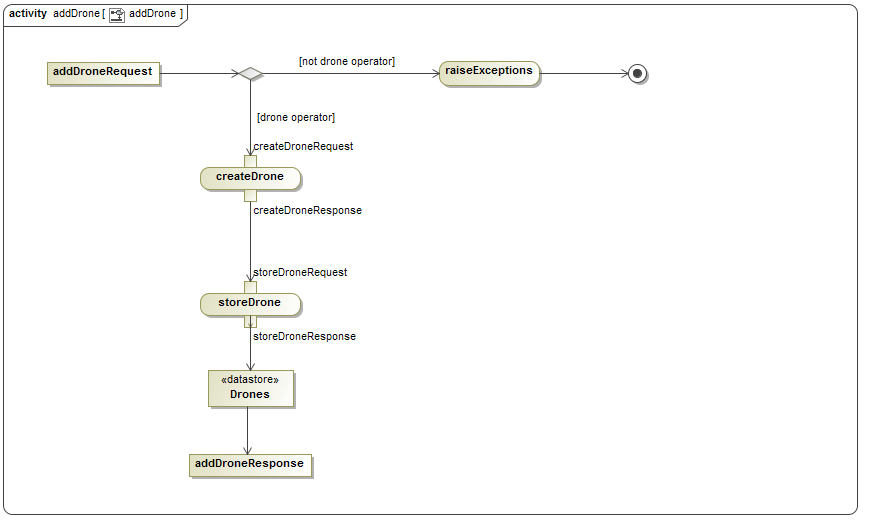
\includegraphics[width=\textwidth]{ps_add.png}  \\
			\caption{Process Specification : addDrone}
		\end{figure}
		\begin{figure}[H]
			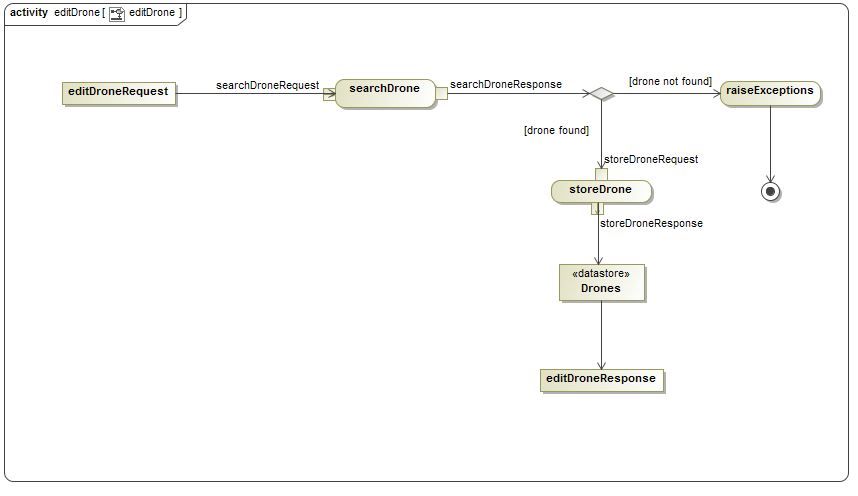
\includegraphics[width=\textwidth]{ps_edit.png}  \\
			\caption{Process Specification : editDrone}
		\end{figure}
		\begin{figure}[H]
			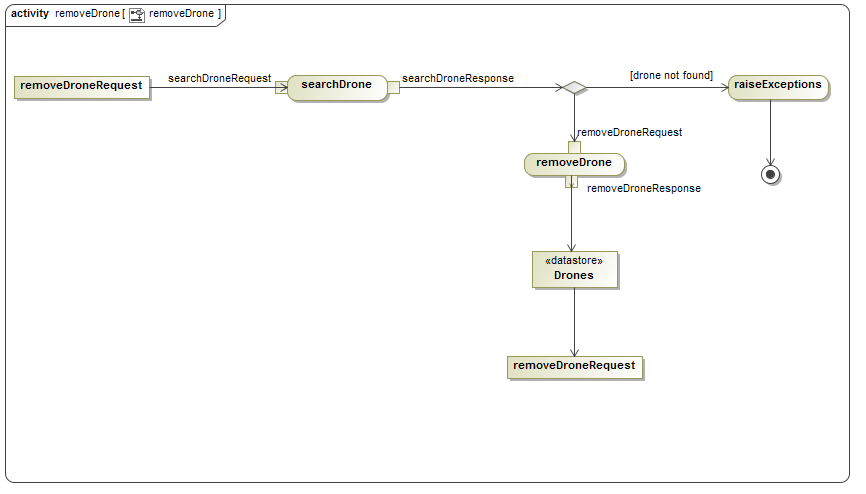
\includegraphics[width=\textwidth]{ps_delete.png}  \\
			\caption{Process Specification : removeDrone}
		\end{figure}
		%To include diagrams for process specifications here.
		
	
	
\newpage

\section{Mission subsection}
%\lable{sec:open}
\subsubsection{Use cases}
	The mission subsection consists if 3 critical functions namely add, delete and view mission. Edit mission is considered a nice to have.
		\begin{flushleft}
			\textbf{Critical}
				\begin{itemize}
	  				\item Add mission
	  				\item Delete mission
	  				\item View mission
				\end{itemize}
				
				\begin{figure}[H]
					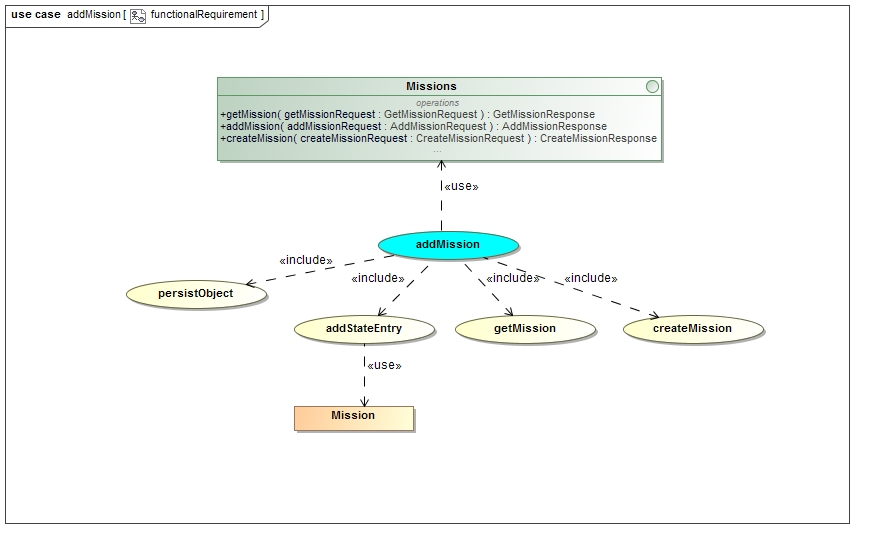
\includegraphics[width=\textwidth]{functionalRequirement_addmission.jpg}  \\
					\caption{Use case : addMission}
				\end{figure}
				
				\begin{figure}[H]
					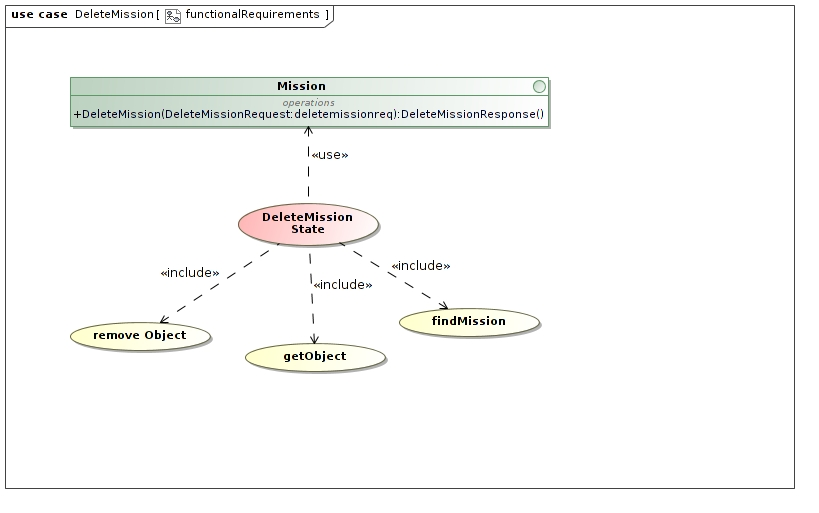
\includegraphics[width=\textwidth]{functionalRequirementsDeleteMission Use Case Diagram.jpg}  \\
					\caption{Use case : deleteMission}
				\end{figure}
				
				\begin{figure}[H]
					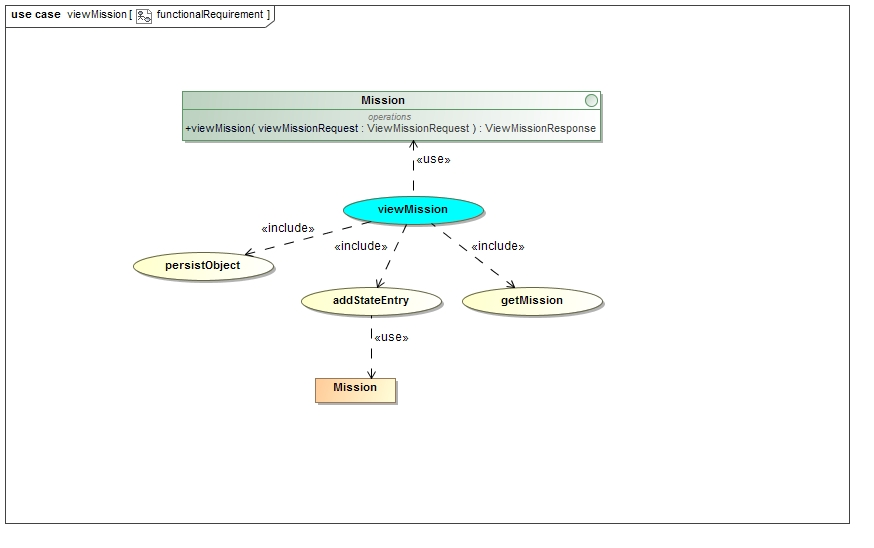
\includegraphics[width=\textwidth]{functionalRequirement_viewmission.jpg}  \\
					\caption{Use case : viewMission}
				\end{figure}

			\textbf{Nice-To-Have}
				\begin{itemize}
	  				\item Edit mission
				\end{itemize}
				
				\begin{figure}[H]
					\includegraphics[width=\textwidth]{functionalRequirementsEditmissin Use case Diagram.jpg}  \\
					\caption{Use case : viewMission}
				\end{figure}
		\end{flushleft}
	\subsection{Service contracts}
	Pre conditions for the service contracts are that only authorized people are allowed to make any changes in the system. Post conditions being changes made to the system mostly in the database.
		\begin{figure}[H]
				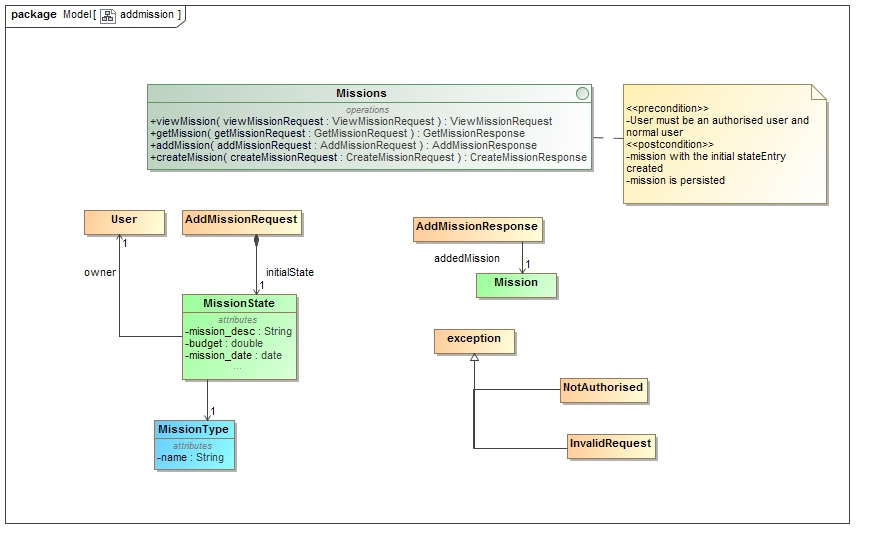
\includegraphics[width=\textwidth]{serviceContract_addmission.jpg}  \\
				\caption{Service contract : addMission}
				\end{figure}
				
		\begin{figure}[H]
				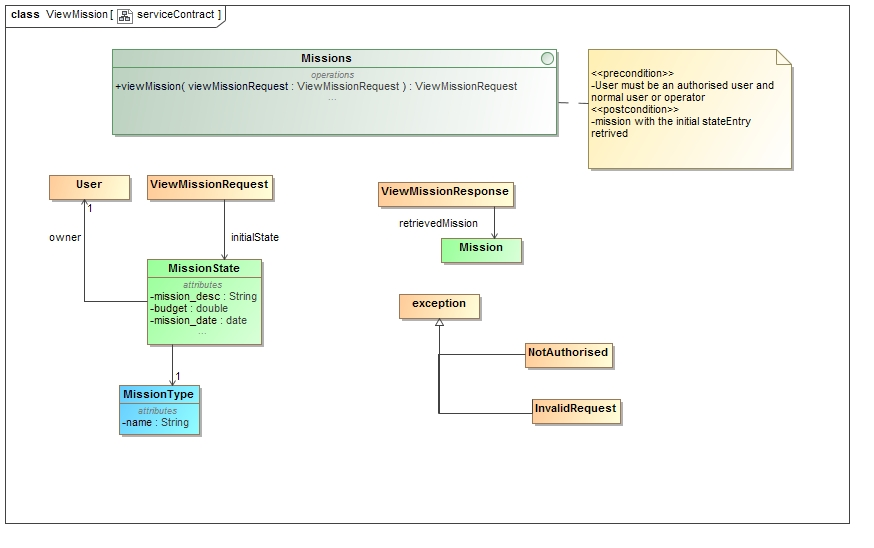
\includegraphics[width=\textwidth]{serviceContract_viewmission.jpg}  \\
				\caption{Service contract : viewMission}
				\end{figure}
				
		\begin{figure}[H]
				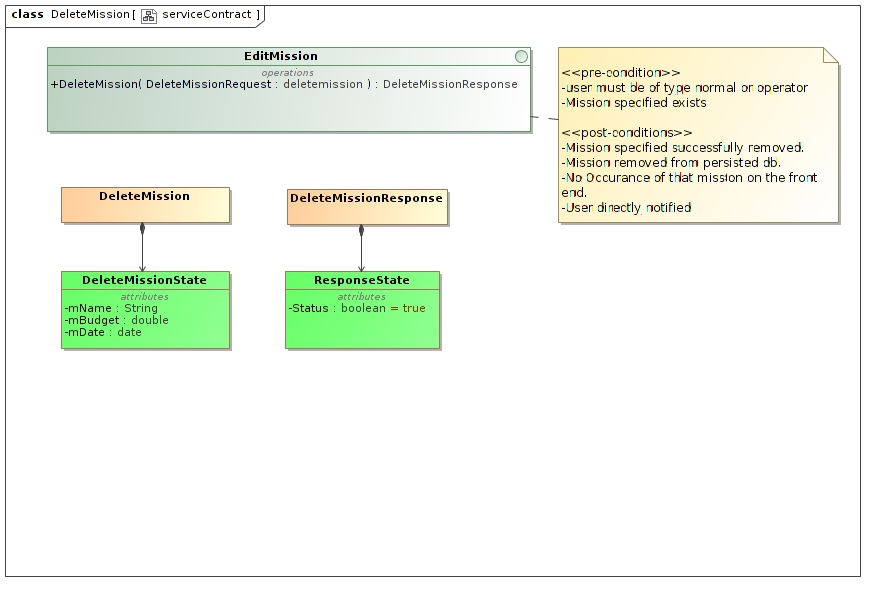
\includegraphics[width=\textwidth]{DeleteMission serviceContract.jpg}  \\
				\caption{Service contract : deleteMission}
				\end{figure}
		\begin{figure}[H]
				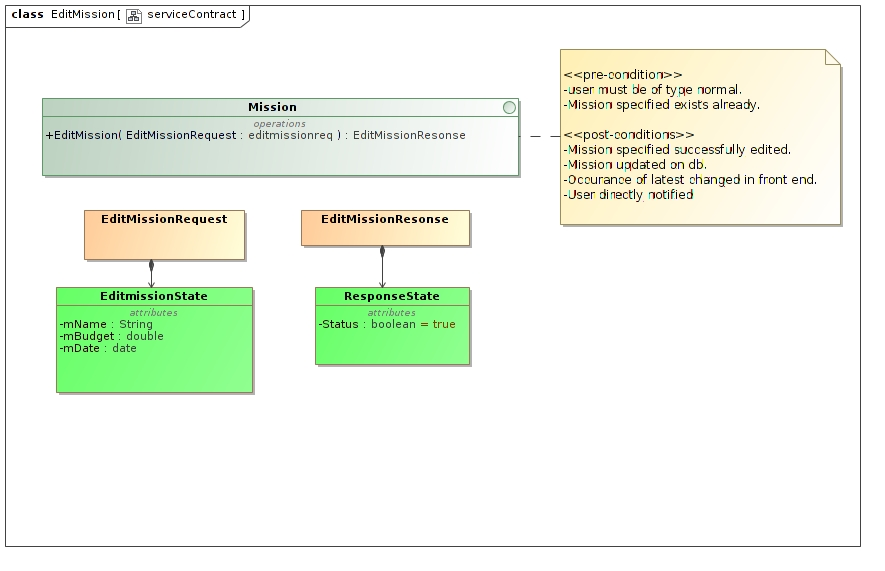
\includegraphics[width=\textwidth]{Edit Mission serviceContract.jpg}  \\
				\caption{Service contract : editMission}
				\end{figure}
				
	\subsection{Process Specifications}
	All missions make additions or removals from the database and can only be made or edited or removed by authorized persons.
		\begin{figure}[H]
				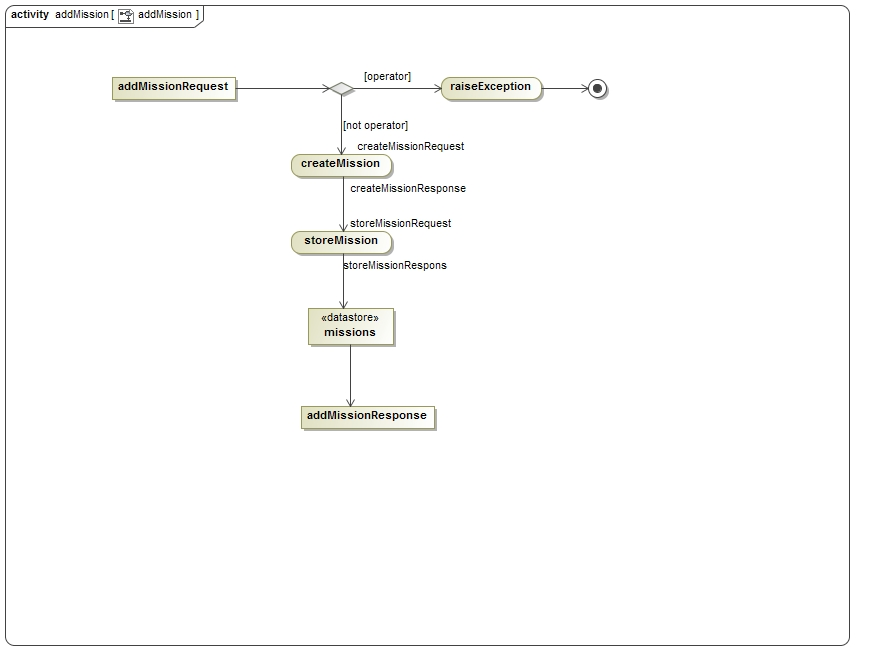
\includegraphics[width=\textwidth]{activity_addmission.jpg}  \\
				\caption{Process specification : addMission}
				\end{figure}
				
		\begin{figure}[H]
				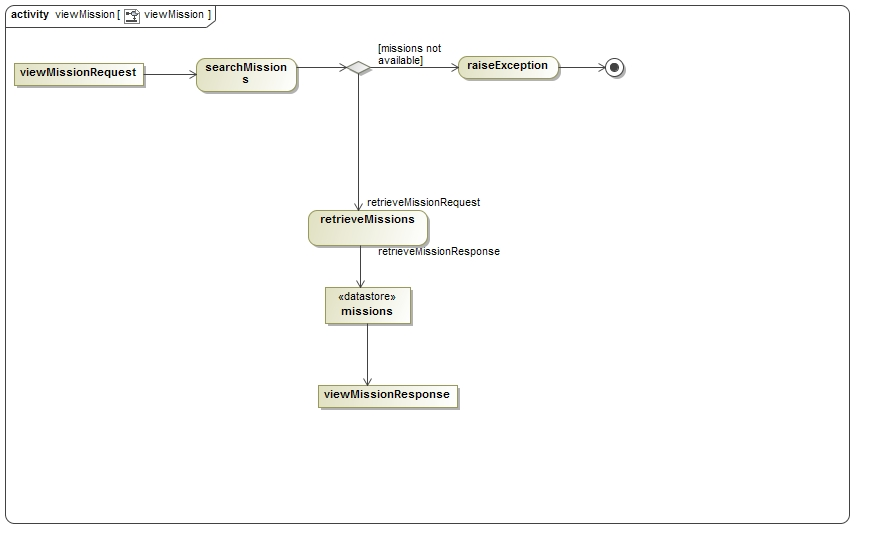
\includegraphics[width=\textwidth]{activity_viewmission.jpg}  \\
				\caption{Process specification : viewMission}
				\end{figure}
				
		\begin{figure}[H]
				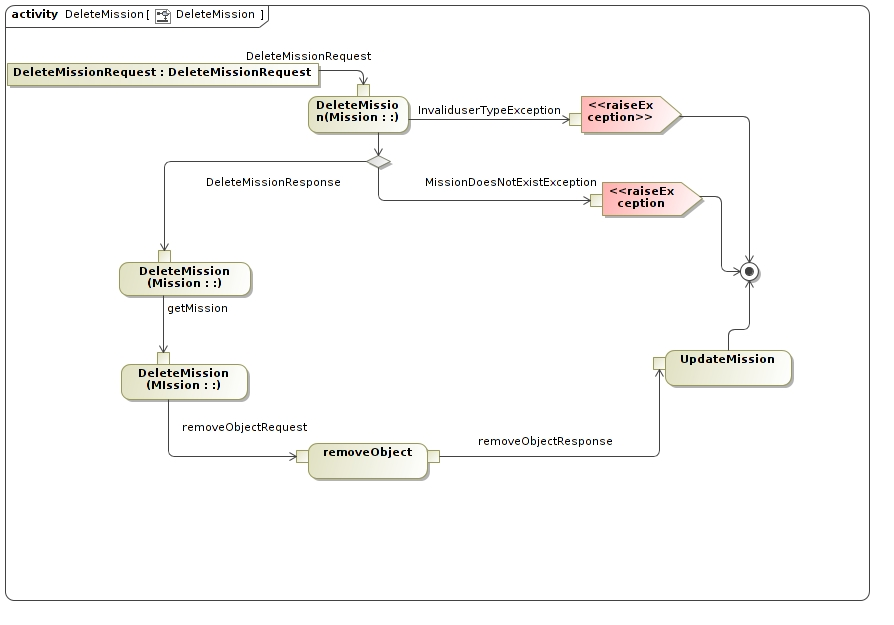
\includegraphics[width=\textwidth]{DeleteMissionActivity diagram.jpg}  \\
				\caption{Process specification : deleteMission}
				\end{figure}
		\begin{figure}[H]
				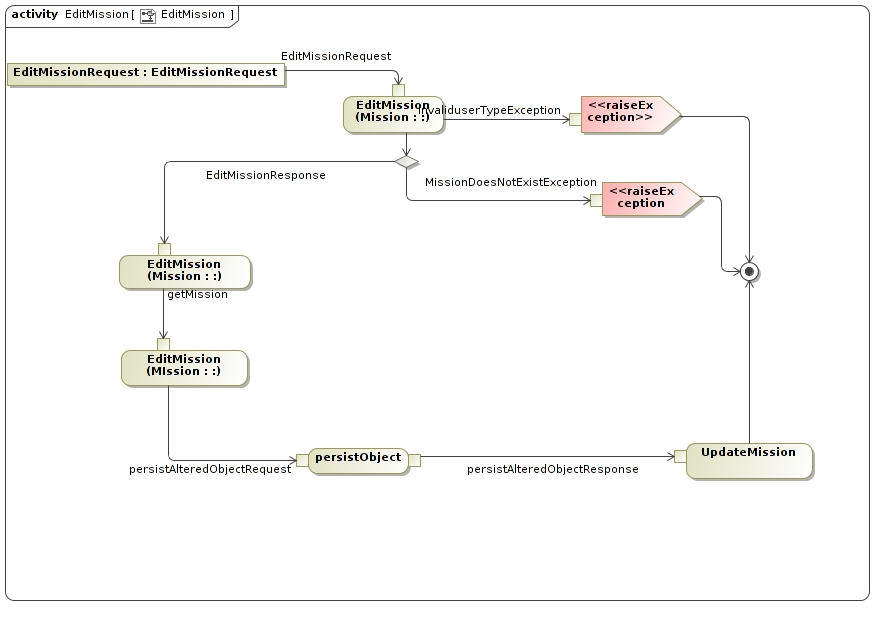
\includegraphics[width=\textwidth]{EditMissionActivityDiagram.jpg}  \\
				\caption{Process specification : editMission}
				\end{figure}
\end{document}
